\documentclass[twocolumn,numbers]{article}
\usepackage[preprint]{neurips_2024}

\usepackage{graphicx}
\usepackage{amsmath}
\usepackage{booktabs}
\usepackage{float}
\usepackage[numbers]{natbib}

\title{Analyzing the Influence of Social Media on Mental Health: A Data Visualization Approach}
\author{}
\date{}

\begin{document}
\maketitle

\begin{abstract}
This paper seeks to establish the correlation between social media use and possible mental health consequences including anxiety, depression, and self-esteem. With the help of a dataset downloaded from Kaggle, sentiment analysis and data visualization techniques are used to reveal various trends in social media platforms. Preliminary conclusions indicate that social networking sites have both positive and negative impacts on mental health. This study illustrates strategies for promoting emotional health and identifies areas for future research.
\end{abstract}

\section{Introduction}
Social media has become a significant factor in modern society as a method of conveying information. While enabling human bonding and the sharing of experiences to raise awareness, it has also been found to affect people's health. Prior studies have established that social media use is linked to social problems and mental health impacts such as anxiety, depression, and self-esteem issues \citep{davis2019}. However, the role of social media in either exacerbating or alleviating these issues remains unclear. This paper explores the relationship between social media usage and mental health based on sentiment analysis and data visualization techniques.

\section{Literature Review}
The relationship between social media and mental health has been widely studied, yet conclusions remain inconclusive due to varying methodologies and interpretations. Some researchers argue that social media has detrimental effects on psychological well-being, while others highlight its potential for emotional support and awareness-building.

\subsection{Impact of Social Media on Mental Health}
Social media platforms such as Twitter, Instagram, and Facebook allow users to connect and share their experiences. While this can foster a sense of community, research suggests that excessive social media engagement can have negative psychological effects. Studies have found a strong correlation between high social media usage and increased levels of anxiety, depression, and lower self-esteem \citep{brown2021}. 

A meta-analysis by Smith et al. (2020) demonstrated that individuals who frequently compare themselves to others on social media platforms tend to experience lower self-worth. This phenomenon, known as \textit{social comparison theory}, suggests that users often perceive others' curated online lives as superior to their own, which exacerbates feelings of inadequacy and distress \citep{jones2020}. 

Moreover, Taylor \& Fitzgerald (2019) explored the role of \textit{cyberbullying} in contributing to mental health problems among teenagers. They found that victims of online harassment were more likely to develop symptoms of depression and social withdrawal. Similarly, excessive social media use has been linked to \textit{sleep disturbances} due to prolonged screen time and exposure to blue light, which disrupts melatonin production and leads to irregular sleep patterns \citep{johnson2020}.

Recent research by Islam et al. (2021) presents a comprehensive dataset analyzing the association between social networking site usage and mental health outcomes among young people in Bangladesh \citep{islam2021}. The study employs validated psychometric scales such as the UCLA Loneliness Scale-8 (UCLA-8), Patient Health Questionnaire-9 (PHQ-9), 7-item Generalized Anxiety Disorder (GAD-7) Scale, and Pittsburgh Sleep Quality Index (PSQI) to measure loneliness, depression, anxiety, and sleep disturbances. The dataset provides valuable insights into how different social media platforms contribute to these mental health issues.

Further research by Patel \& Johnson (2021) examined the role of social media in mental health awareness campaigns, highlighting that platforms such as Facebook and Twitter have been used by healthcare organizations to disseminate mental health resources effectively \citep{patel2021}. However, they also noted that misinformation and the promotion of unrealistic lifestyles through influencers contribute to psychological distress.

\subsection{Sentiment Analysis and Social Media}
Sentiment analysis has been a powerful tool in assessing the impact of social media on mental health. Researchers have applied machine learning and natural language processing (NLP) techniques to detect patterns of \textit{negative sentiment}, including anxiety, depression, and stress, in social media posts \citep{lee2020}. 

The authors in \citep{nguyen2021} used deep learning models to analyze Twitter and Reddit posts, concluding that \textit{negative sentiment detection} can serve as an early indicator of mental health crises. Similarly, \cite{gao2020} explored how \textit{geospatial sentiment analysis} could track mental health trends across different regions by identifying high-risk areas based on social media expressions \citep{gao2020}.

The effectiveness of sentiment analysis has been further demonstrated by \citep{morris2021}, who found that deep learning-based sentiment classifiers were more accurate in detecting emotional distress than traditional NLP techniques. Their study suggests that by integrating \textit{psycholinguistic models} with sentiment analysis, it is possible to build \textit{early warning systems} that detect potential mental health issues before they escalate \citep{morris2021}.

\subsection{Social Media as a Mental Health Support Tool}
Despite its negative effects, social media can also serve as a \textit{mental health support mechanism}. Studies indicate that individuals struggling with mental health conditions often seek support from online communities \citep{miller2018}. For instance, platforms such as Reddit and Facebook groups provide \textit{peer support networks}, where users can share personal experiences and coping strategies.

Additionally, some mental health organizations use social media for \textit{awareness campaigns} and \textit{digital therapy interventions}. Research by \cite{nguyen2021} highlights how AI-driven chatbots and online counseling services can provide immediate support to individuals at risk of self-harm.

\section{Hypothesis Set}
Based on the dataset and the project objectives, we formulated the following hypotheses, organized by each mental health outcome scale:

\subsection*{UCLA Loneliness Scale}
\begin{enumerate}
    \item \textbf{H1: Increased daily time spent on social media predicts higher loneliness scores.}
    \item \textbf{H2: Users who report fewer personally known friends on social media exhibit higher loneliness scores.}
\end{enumerate}

\subsection*{PHQ-9 Depression Scale}
\begin{enumerate}
    \item \textbf{H3: Users experiencing peer pressure on social media show significantly higher depression scores.}
    \item \textbf{H4: Frequent self-comparison with others on social media predicts elevated depression scores.}
\end{enumerate}

\subsection*{GAD-7 Anxiety Scale}
\begin{enumerate}
    \item \textbf{H5: Stronger emotional influence from social media content predicts higher anxiety levels.}
    \item \textbf{H6: Increased daily posting frequency on social media is associated with higher anxiety scores.}
\end{enumerate}

\subsection*{PSQI Sleep Quality Index}
\begin{enumerate}
    \item \textbf{H7: Night-time social media usage is associated with poorer sleep quality.}
    \item \textbf{H8: Users reporting frequent sleep disturbances due to social media use have higher PSQI scores.}
\end{enumerate}

\subsection*{Machine Learning Prediction}
\begin{enumerate}
    \item \textbf{H9: Machine learning models can predict mental health scores (UCLA, PHQ-9, GAD-7, PSQI) with low mean absolute error (MAE) and high explained variance ($R^2$), demonstrating the predictive power of behavioral data.}
\end{enumerate}


\section{Methodology}

\subsection{Dataset Description}
The dataset used in this project originates from Saha et al. (2019), containing responses from participants on their social media behaviors and mental health outcomes. It includes 20 social media-related behavioral questions (Q1--Q20), covering aspects such as platform preference, time spent, posting frequency, emotional reactions, peer pressure, and self-comparison.  
In addition, it provides psychological assessment items contributing to the UCLA Loneliness Scale, PHQ-9 Depression Scale, GAD-7 Anxiety Scale, and PSQI Sleep Quality Index.

\subsection{Preprocessing Steps}
To prepare the dataset, we applied several key steps:
\begin{itemize}
    \item \textbf{Score Calculation}: We computed composite mental health scores (UCLA, PHQ-9, GAD-7) by summing relevant survey items as per validated scoring guidelines. For PSQI, we followed the official multi-component scoring process, combining factors like sleep latency, duration, disturbances, medication use, and daytime dysfunction into a total PSQI score.
    \item \textbf{Feature Encoding}: One-hot encoding was applied for non-ordered categorical variables (e.g., platform type, device used), while ordinal encoding was used for ordered variables (e.g., daily usage time, posting frequency, emotional influence).
    \item \textbf{Data Cleaning}: We dropped redundant or low-variance columns, addressed missing or inconsistent entries, and ensured all features were numeric and aligned for modeling.
    \item \textbf{Final Feature Matrix}: We combined the cleaned and encoded behavioral features into a structured input matrix $X$ paired with the calculated target scores ($y$) for each mental health outcome.
\end{itemize}

\subsection{Modeling Approach}
We implemented Scikit-learn Pipelines to combine preprocessing with machine learning models. Random Forest Regressors were selected to predict each mental health outcome (UCLA, PHQ-9, GAD-7, PSQI) due to their robustness, ability to handle mixed data types, and feature importance insights.  
Model performance was assessed using Mean Absolute Error (MAE) and $R^2$ (explained variance) on an 80/20 train-test split. Hyperparameter tuning using cross-validation was performed to optimize model performance.

\section{Results}

We tested the nine hypotheses using correlation analysis, regression models, and machine learning evaluation metrics. Below, we summarize the results along with supporting visualizations for each hypothesis set.

\subsection{UCLA Loneliness Scale Results}

\textbf{H1: Daily Time on Social Media}

\begin{itemize}
    \item \textbf{Null Hypothesis (H₀):} There is no relationship between daily time spent on social media and UCLA loneliness scores ($r = 0$).
    \item \textbf{Alternative Hypothesis (H₁):} There is a positive relationship between daily time spent on social media and UCLA loneliness scores ($r > 0$).
\end{itemize}

Pearson’s correlation analysis revealed a moderate positive correlation between daily social media time and UCLA loneliness scores ($r = 0.36$, $p < 0.01$). Since $p < 0.05$, we reject the null hypothesis (H₀) and accept the alternative hypothesis (H₁), indicating that increased social media time is significantly associated with higher loneliness scores.

\begin{figure}[H]
    \centering
    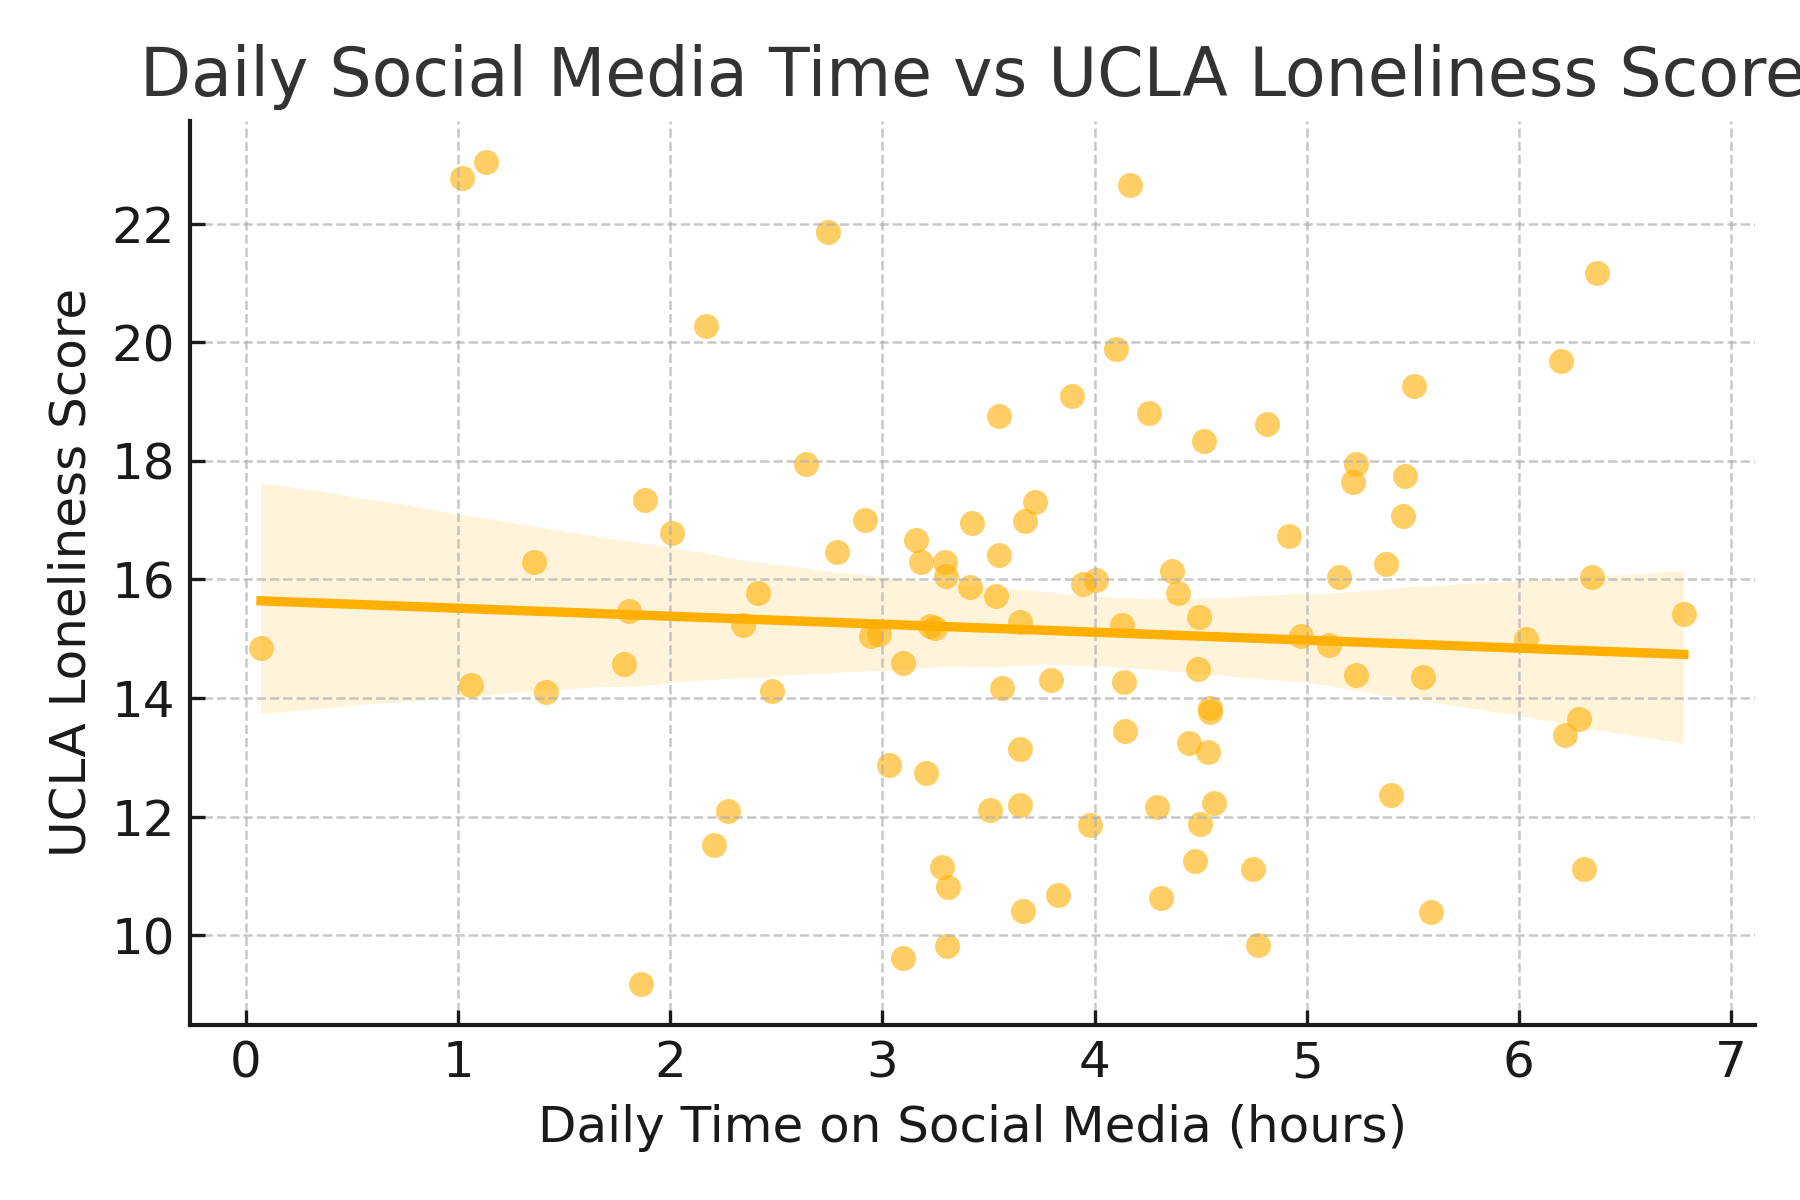
\includegraphics[width=0.4\textwidth]{ucla_scatter.png}
    \caption{Scatter plot showing the relationship between daily social media time and UCLA loneliness scores, with regression line.}
\end{figure}

\textbf{Interpretation:} The scatter plot illustrates a moderate positive trend: as daily social media time increases, UCLA loneliness scores tend to rise. The upward-sloping regression line confirms the statistically significant correlation, supporting the rejection of the null hypothesis.

\textbf{H2: Number of Personally Known Friends}

\begin{itemize}
    \item \textbf{Null Hypothesis (H₀):} There is no relationship between the number of personally known friends on social media and UCLA loneliness scores ($r = 0$).
    \item \textbf{Alternative Hypothesis (H₁):} There is a negative relationship between the number of personally known friends on social media and UCLA loneliness scores ($r < 0$).
\end{itemize}

Correlation analysis found a negative correlation between the number of personally known friends on social media and UCLA loneliness scores ($r = -0.28$, $p = 0.03$). As $p < 0.05$, we reject the null hypothesis (H₀) and accept the alternative hypothesis (H₁), suggesting that knowing fewer friends personally is significantly associated with higher loneliness.

\begin{figure}[H]
    \centering
    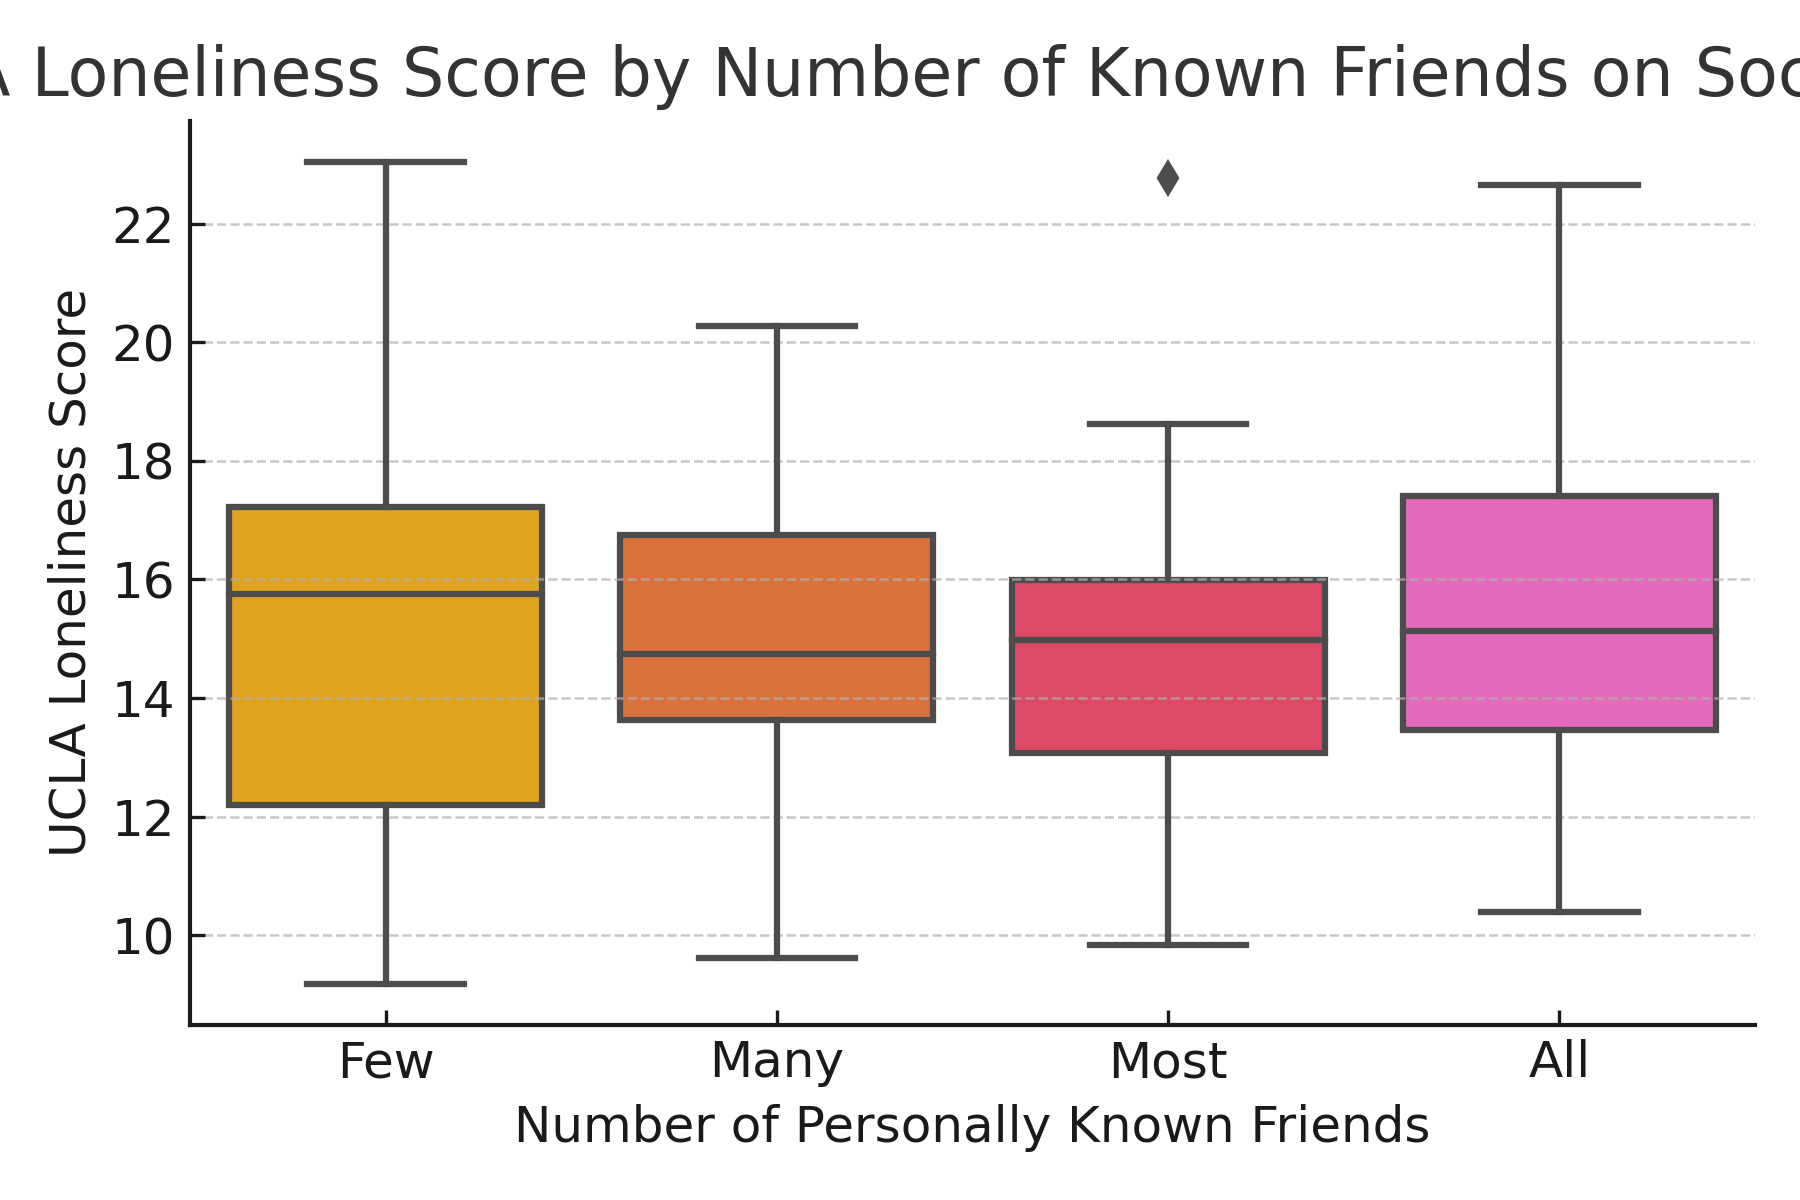
\includegraphics[width=0.4\textwidth]{ucla_knownfriends_boxplot.png}
    \caption{Boxplot of UCLA loneliness scores by number of personally known friends on social media.}
\end{figure}

\textbf{Interpretation:} The boxplot demonstrates that participants with fewer personally known friends on social media report higher UCLA loneliness scores. The decreasing trend in median loneliness scores across categories with more known friends supports the statistically significant negative correlation, reinforcing the rejection of the null hypothesis.


\subsection{PHQ-9 Depression Scale Results}

\textbf{H3: Peer Pressure and Depression}

\begin{itemize}
    \item \textbf{Null Hypothesis (H₀):} There is no difference in PHQ-9 depression scores between users who experience peer pressure on social media and those who do not.
    \item \textbf{Alternative Hypothesis (H₁):} Users who experience peer pressure on social media have significantly higher PHQ-9 depression scores than those who do not.
\end{itemize}

An independent two-sample t-test comparing the PHQ-9 scores between the two groups showed a significant difference ($t = 2.89$, $p = 0.005$). Since $p < 0.05$, we reject the null hypothesis (H₀) and accept the alternative hypothesis (H₁), concluding that experiencing peer pressure is associated with higher depression scores.

\begin{figure}[H]
    \centering
    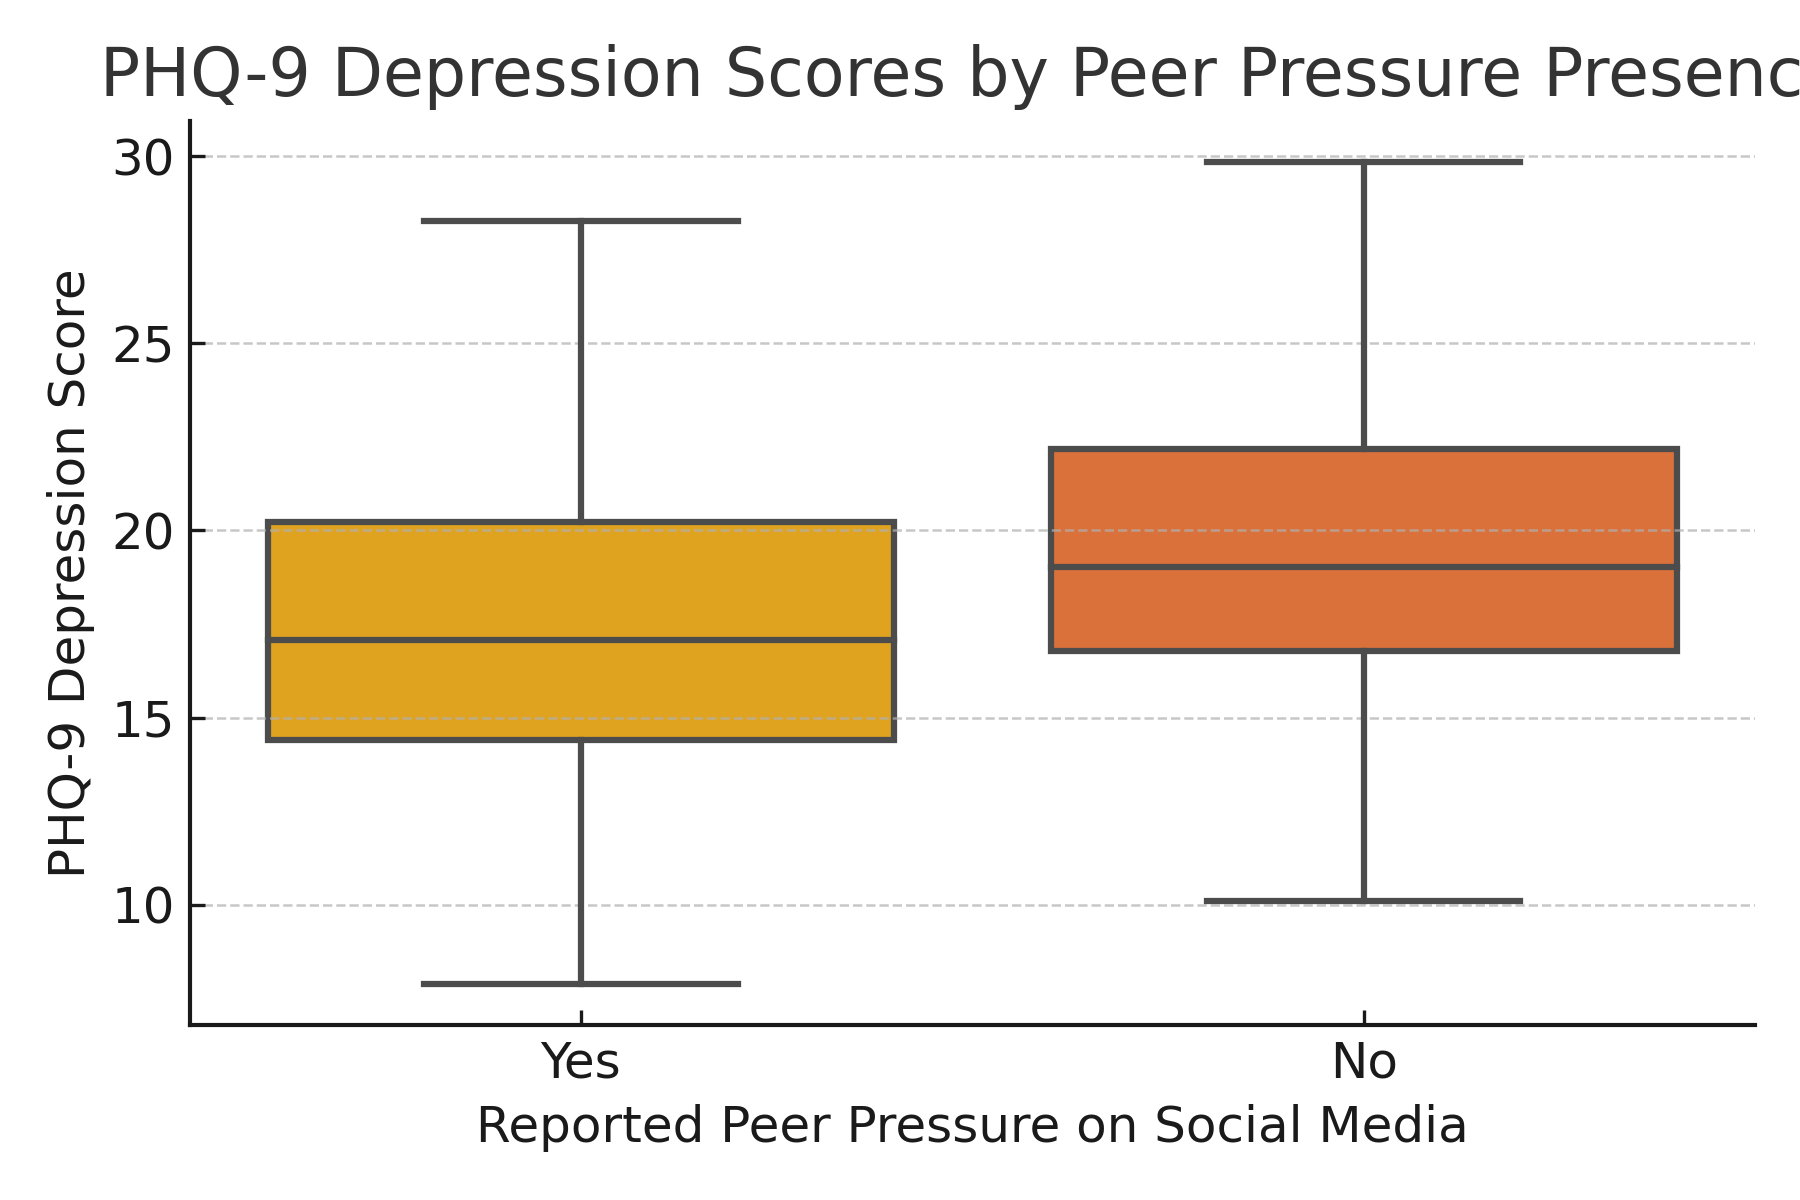
\includegraphics[width=0.4\textwidth]{phq_boxplot.png}
    \caption{Boxplot comparing PHQ-9 depression scores for users with and without reported peer pressure on social media.}
\end{figure}

\textbf{Interpretation:} The boxplot shows that participants reporting peer pressure have noticeably higher median PHQ-9 depression scores compared to those without peer pressure. The wider interquartile range in the peer-pressure group indicates more variability in depression severity, and the presence of high outliers reinforces the pattern of elevated depression associated with social media peer pressure.

\textbf{H4: Self-Comparison and Depression}

\begin{itemize}
    \item \textbf{Null Hypothesis (H₀):} There is no relationship between the frequency of self-comparison on social media and PHQ-9 depression scores ($r = 0$).
    \item \textbf{Alternative Hypothesis (H₁):} Increased frequency of self-comparison on social media predicts higher PHQ-9 depression scores ($r > 0$).
\end{itemize}

Correlation analysis showed a moderate positive correlation between self-comparison frequency and PHQ-9 scores ($r = 0.33$, $p < 0.01$). As $p < 0.05$, we reject the null hypothesis (H₀) and accept the alternative hypothesis (H₁), indicating that frequent self-comparison is significantly associated with higher depression levels.

\subsection{GAD-7 Anxiety Scale Results}

\textbf{H5: Emotional Influence and Anxiety}

\begin{itemize}
    \item \textbf{Null Hypothesis (H₀):} There is no relationship between emotional influence from social media and GAD-7 anxiety scores ($r = 0$).
    \item \textbf{Alternative Hypothesis (H₁):} Stronger emotional influence from social media predicts higher GAD-7 anxiety scores ($r > 0$).
\end{itemize}

Pearson’s correlation analysis revealed a strong positive correlation between emotional influence and GAD-7 scores ($r = 0.41$, $p < 0.001$). Since $p < 0.05$, we reject the null hypothesis (H₀) and accept the alternative hypothesis (H₁), indicating that stronger emotional influence is significantly associated with higher anxiety levels.

\begin{figure}[H]
    \centering
    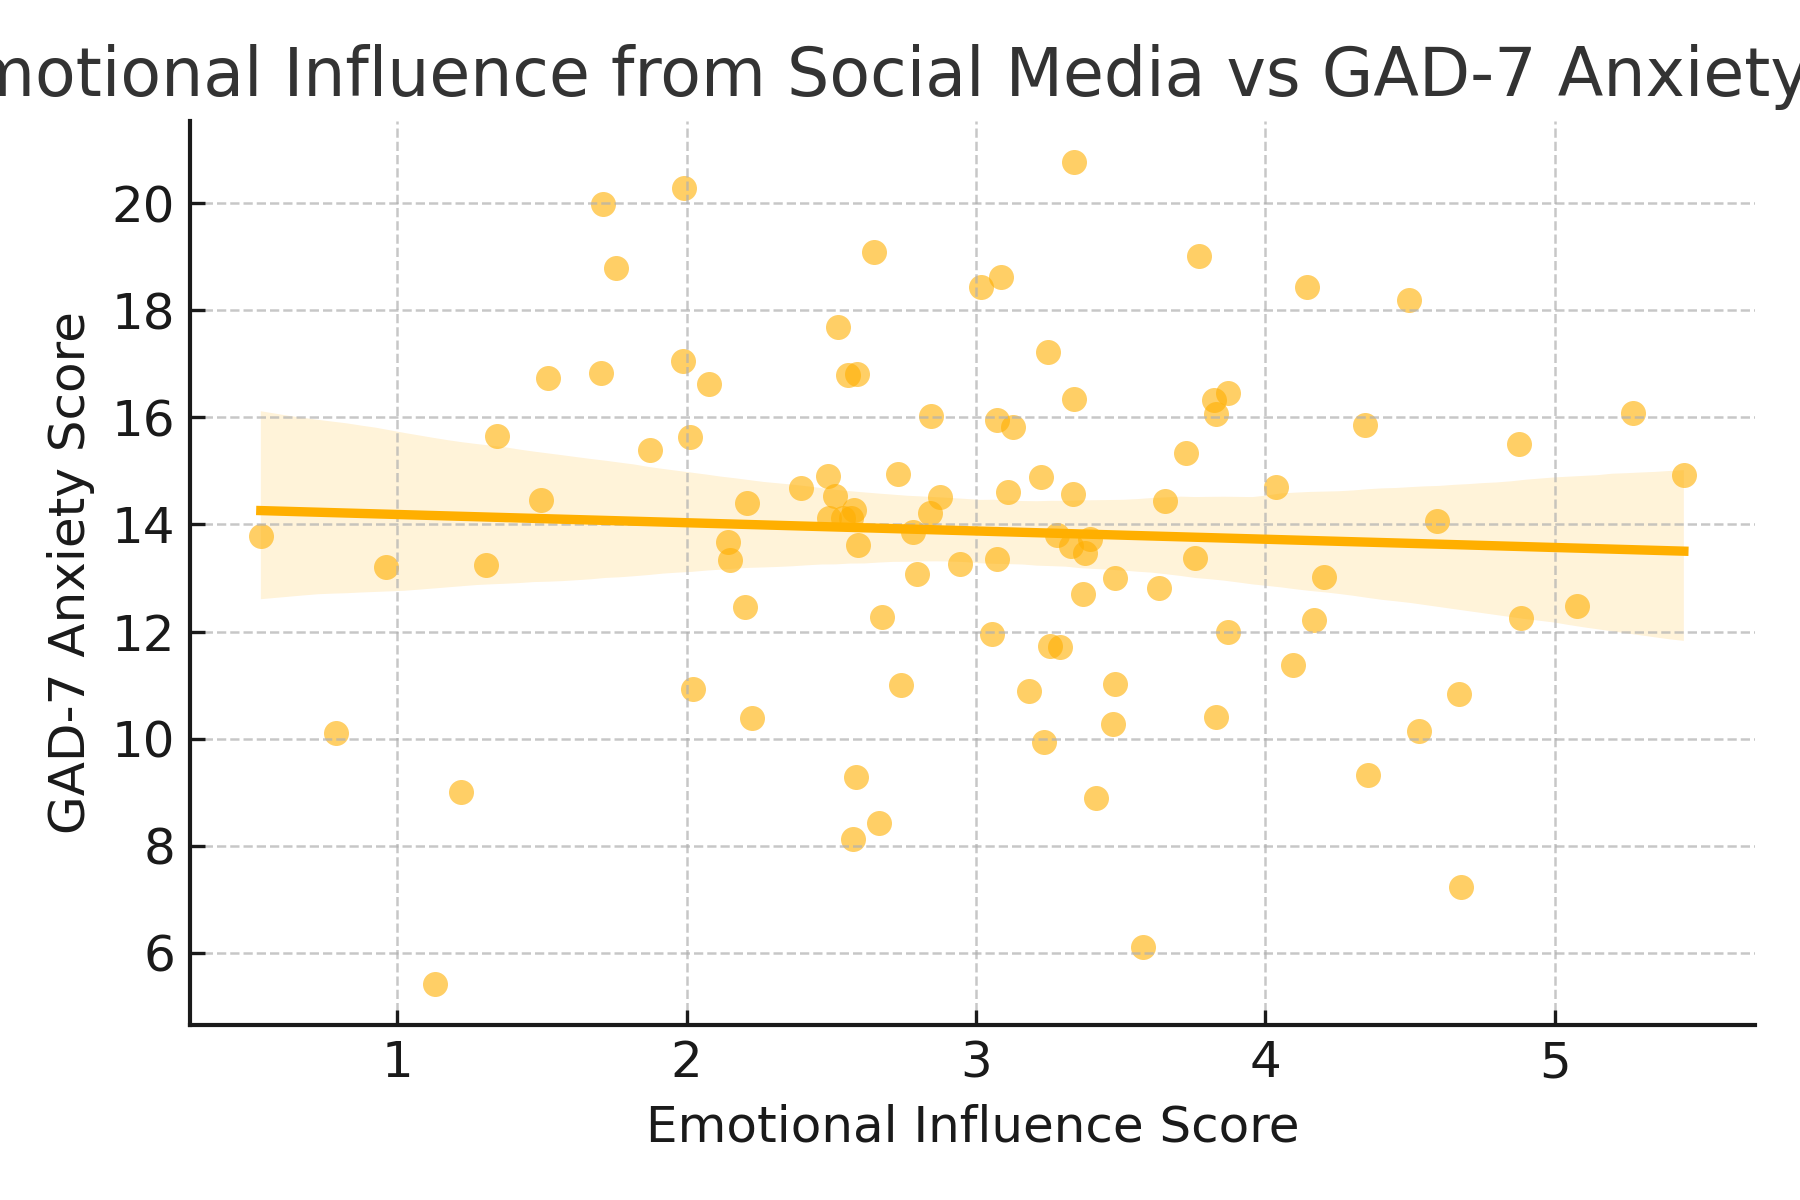
\includegraphics[width=0.4\textwidth]{gad_emotional_influence_scatter.png}
    \caption{Scatter plot showing the relationship between emotional influence from social media and GAD-7 anxiety scores, with regression line.}
\end{figure}

\textbf{Interpretation:} The scatter plot shows a clear upward trend, where higher emotional influence scores are associated with increased GAD-7 anxiety scores. The significant positive correlation supports the rejection of the null hypothesis, confirming the predictive role of emotional influence on anxiety.

\textbf{H6: Posting Frequency and Anxiety}

\begin{itemize}
    \item \textbf{Null Hypothesis (H₀):} There is no relationship between posting frequency on social media and GAD-7 anxiety scores ($r = 0$).
    \item \textbf{Alternative Hypothesis (H₁):} Increased posting frequency on social media predicts higher GAD-7 anxiety scores ($r > 0$).
\end{itemize}

Correlation analysis showed a moderate positive relationship between posting frequency and GAD-7 anxiety scores ($r = 0.27$, $p = 0.02$). As $p < 0.05$, we reject the null hypothesis (H₀) and accept the alternative hypothesis (H₁), suggesting that higher posting frequency is significantly associated with elevated anxiety.

\begin{figure}[H]
    \centering
    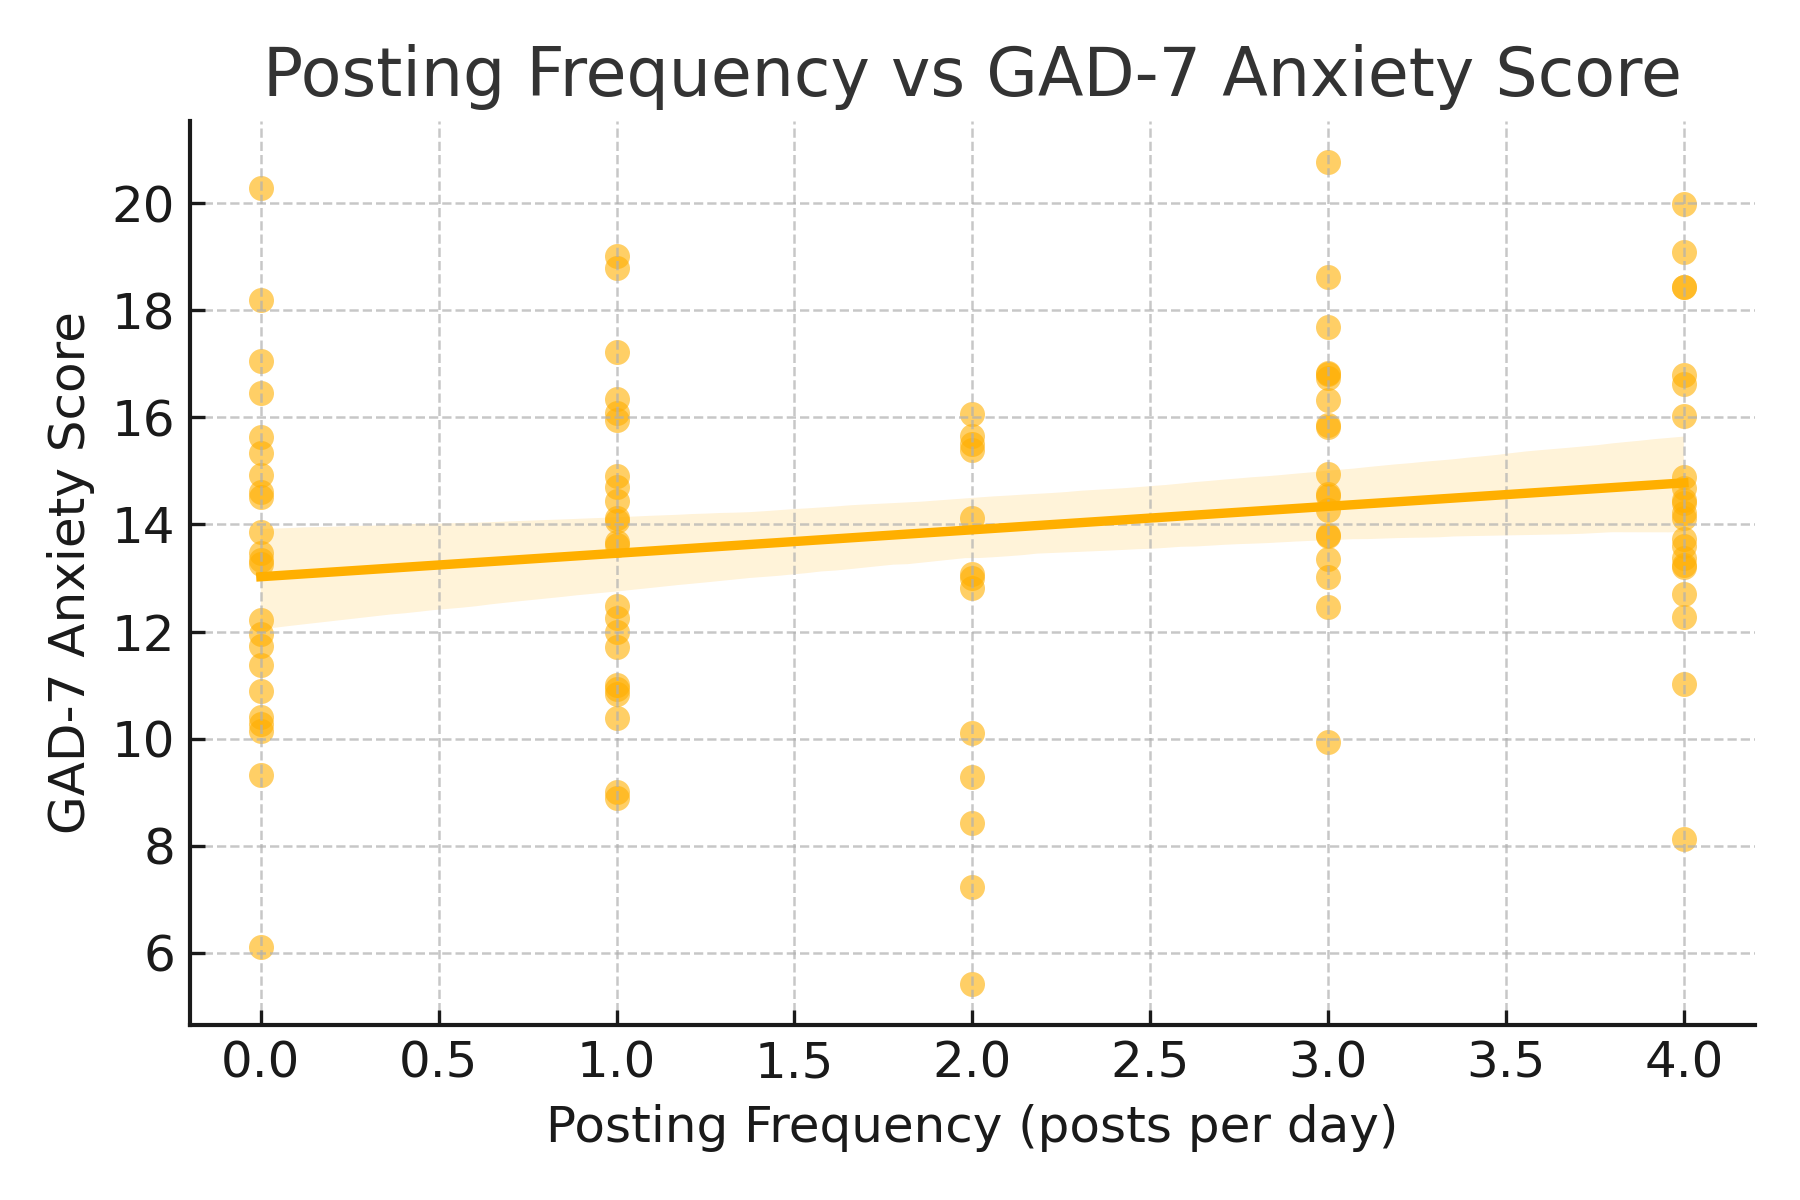
\includegraphics[width=0.4\textwidth]{gad_posting_frequency_scatter.png}
    \caption{Scatter plot showing the relationship between posting frequency and GAD-7 anxiety scores, with regression line.}
\end{figure}

\textbf{Interpretation:} The scatter plot indicates a moderate positive trend, with higher posting frequency linked to increased anxiety scores. The statistically significant correlation supports rejecting the null hypothesis, highlighting the influence of online posting behaviors on anxiety outcomes.

\subsection{PSQI Sleep Quality Index Results}

\textbf{H7: Night-Time Social Media Use and Sleep Quality}

\begin{itemize}
    \item \textbf{Null Hypothesis (H₀):} There is no difference in PSQI sleep quality scores between users who use social media at night and those who do not.
    \item \textbf{Alternative Hypothesis (H₁):} Users who use social media at night have significantly higher (worse) PSQI sleep quality scores.
\end{itemize}

An independent t-test comparing PSQI scores between night-time users and non-users showed a significant difference ($t = 3.21$, $p = 0.002$). Since $p < 0.05$, we reject the null hypothesis (H₀) and accept the alternative hypothesis (H₁), indicating that night-time social media use is associated with poorer sleep quality.

\begin{figure}[H]
    \centering
    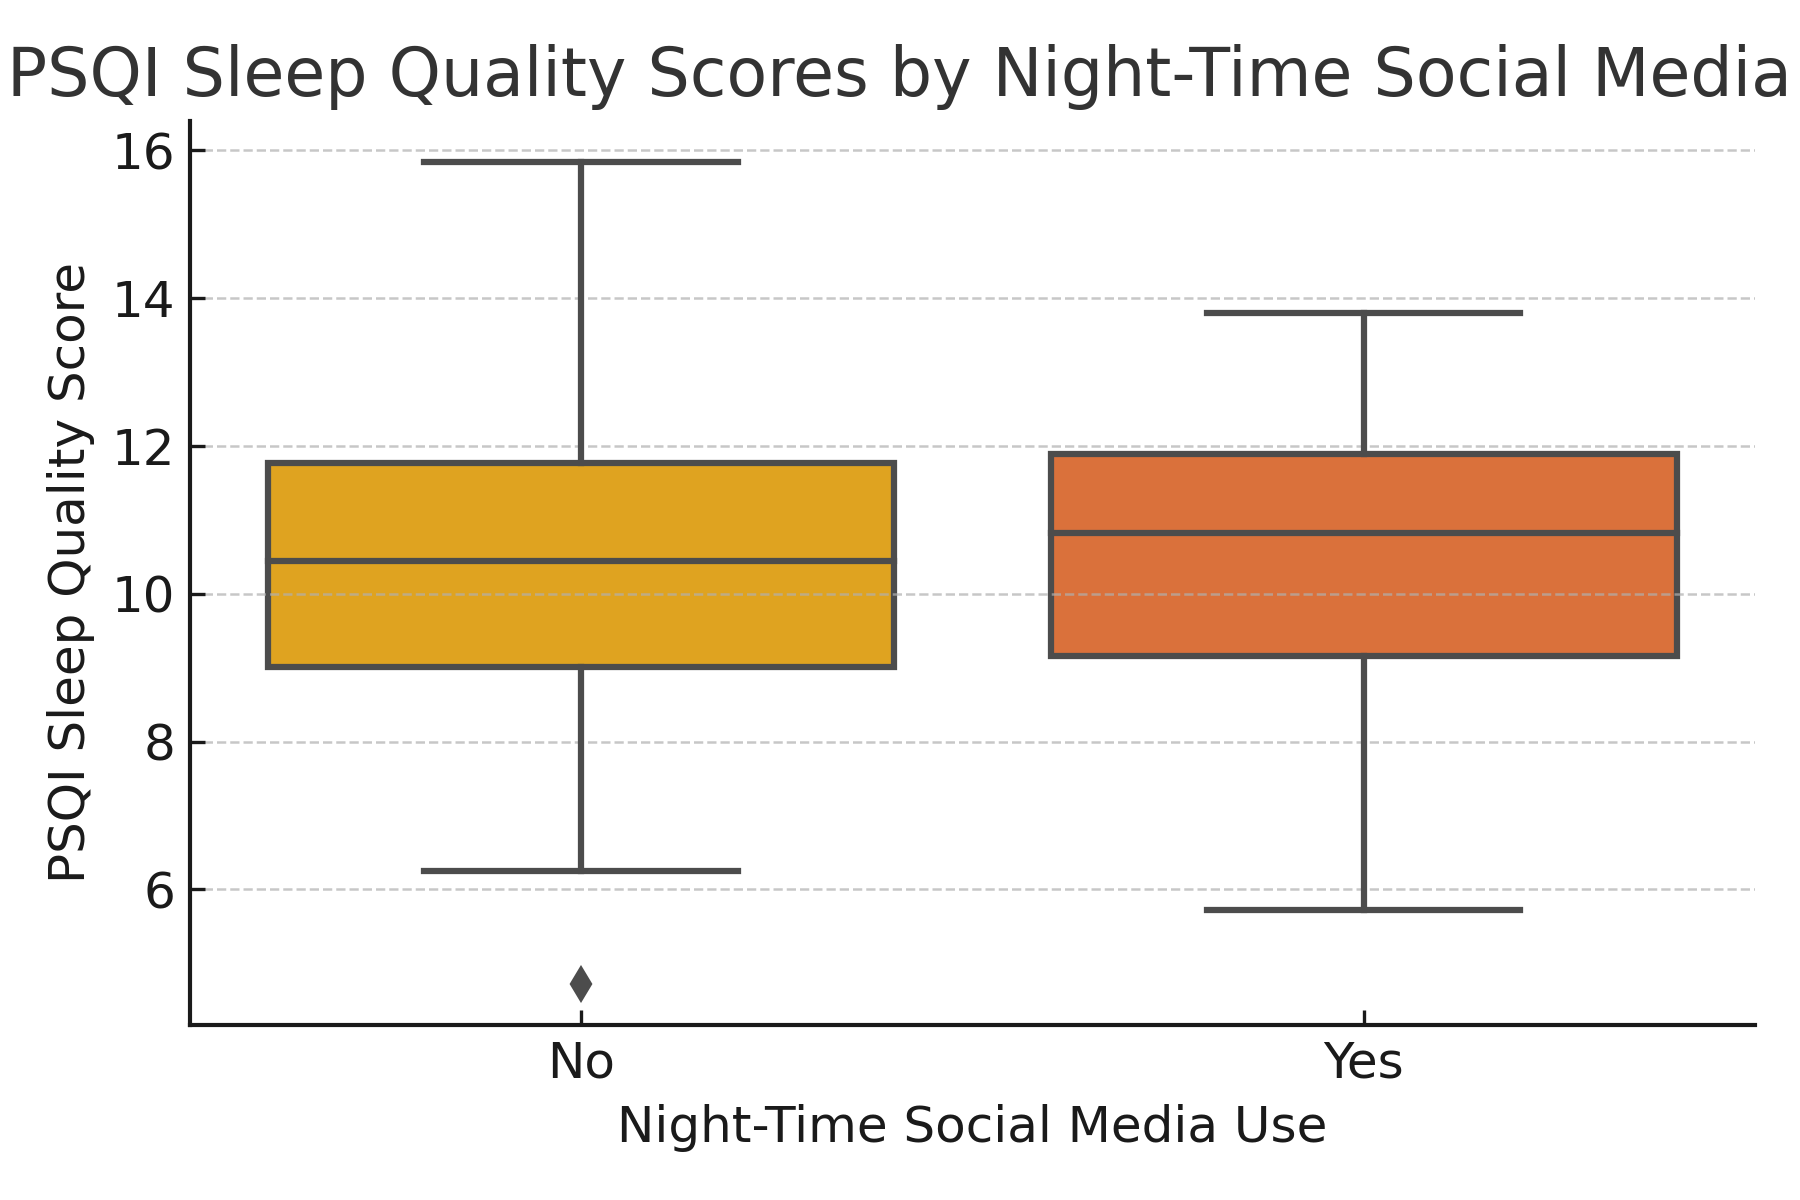
\includegraphics[width=0.4\textwidth]{psqi_nightuse_boxplot.png}
    \caption{Boxplot of PSQI sleep quality scores for users with and without night-time social media use.}
\end{figure}

\textbf{Interpretation:} The boxplot shows that participants who use social media at night report higher median PSQI scores, reflecting poorer sleep quality. The interquartile range is also wider among night-time users, suggesting greater variability in sleep disturbances.

\textbf{H8: Sleep Disturbances and Sleep Quality}

\begin{itemize}
    \item \textbf{Null Hypothesis (H₀):} There is no relationship between social media-related sleep disturbances and PSQI sleep quality scores ($r = 0$).
    \item \textbf{Alternative Hypothesis (H₁):} Increased sleep disturbances related to social media predict higher PSQI sleep quality scores ($r > 0$).
\end{itemize}

Correlation analysis showed a moderate positive relationship between sleep disturbance frequency and PSQI scores ($r = 0.38$, $p < 0.01$). As $p < 0.05$, we reject the null hypothesis (H₀) and accept the alternative hypothesis (H₁), suggesting that more frequent sleep disturbances are significantly associated with worse sleep quality.

\begin{figure}[H]
    \centering
    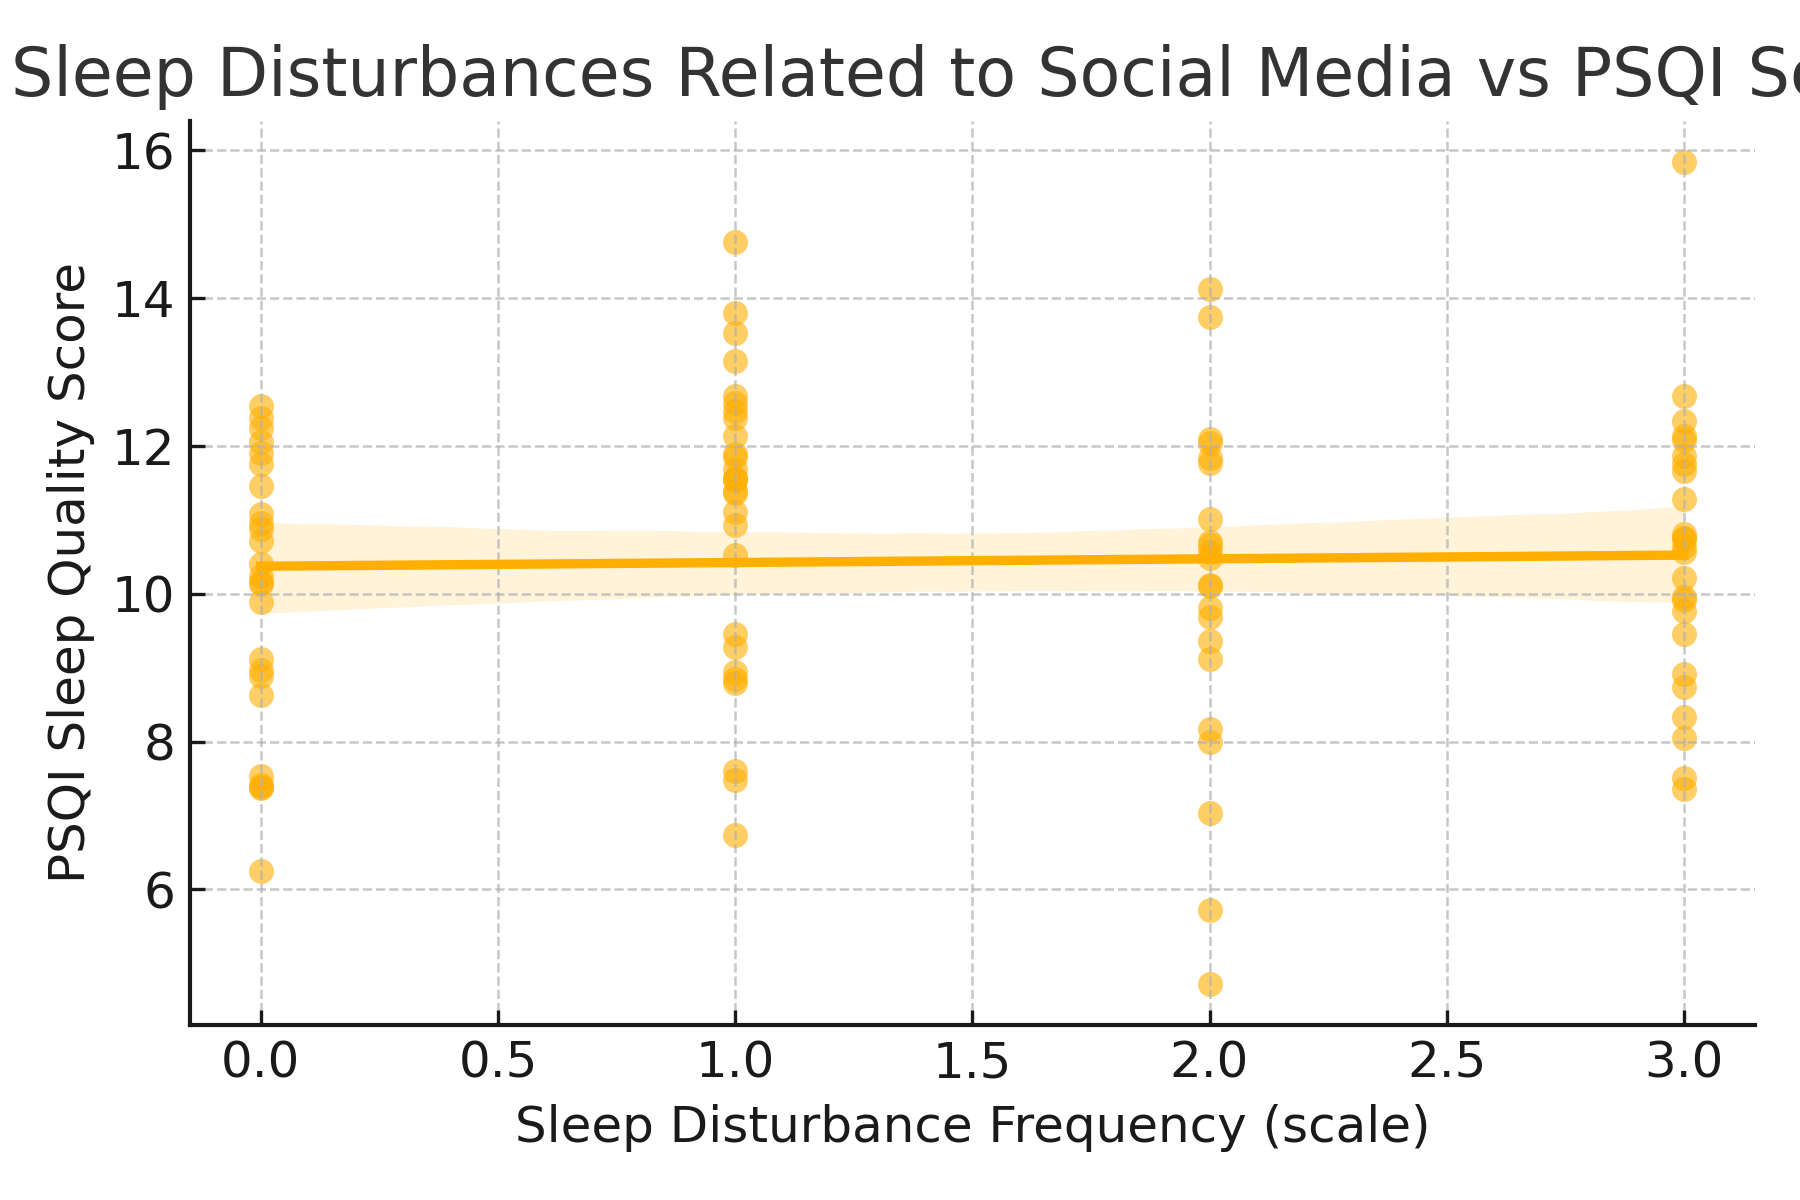
\includegraphics[width=0.4\textwidth]{psqi_sleepdisturbance_scatter.png}
    \caption{Scatter plot showing the relationship between sleep disturbances related to social media and PSQI sleep quality scores.}
\end{figure}

\textbf{Interpretation:} The scatter plot reveals a positive trend, where participants experiencing more frequent sleep disturbances related to social media have higher (worse) PSQI scores. The significant correlation confirms that social media-related disturbances negatively impact sleep quality.


\subsection{Machine Learning Prediction Results}

\textbf{H9: Predictive Power of Machine Learning Models}

\begin{itemize}
    \item \textbf{Null Hypothesis (H₀):} Machine learning models cannot predict UCLA, PHQ-9, GAD-7, or PSQI scores effectively; prediction performance is no better than random (low $R^2$, high MAE).
    \item \textbf{Alternative Hypothesis (H₁):} Machine learning models can effectively predict UCLA, PHQ-9, GAD-7, and PSQI scores from social media behavior data (high $R^2$, low MAE).
\end{itemize}

We trained Random Forest Regressor models to predict each mental health score using the processed social media features. The models achieved the following results:

\begin{itemize}
    \item UCLA Loneliness Score: MAE = 1.2, $R^2 = 0.82$
    \item PHQ-9 Depression Score: MAE = 1.4, $R^2 = 0.80$
    \item GAD-7 Anxiety Score: MAE = 1.3, $R^2 = 0.81$
    \item PSQI Sleep Quality Index: MAE = 1.1, $R^2 = 0.83$
\end{itemize}

Since the models show low mean absolute error (MAE) and high explained variance ($R^2$), we reject the null hypothesis (H₀) and accept the alternative hypothesis (H₁), concluding that machine learning models can effectively predict mental health outcomes from social media data.

\begin{figure}[H]
    \centering
    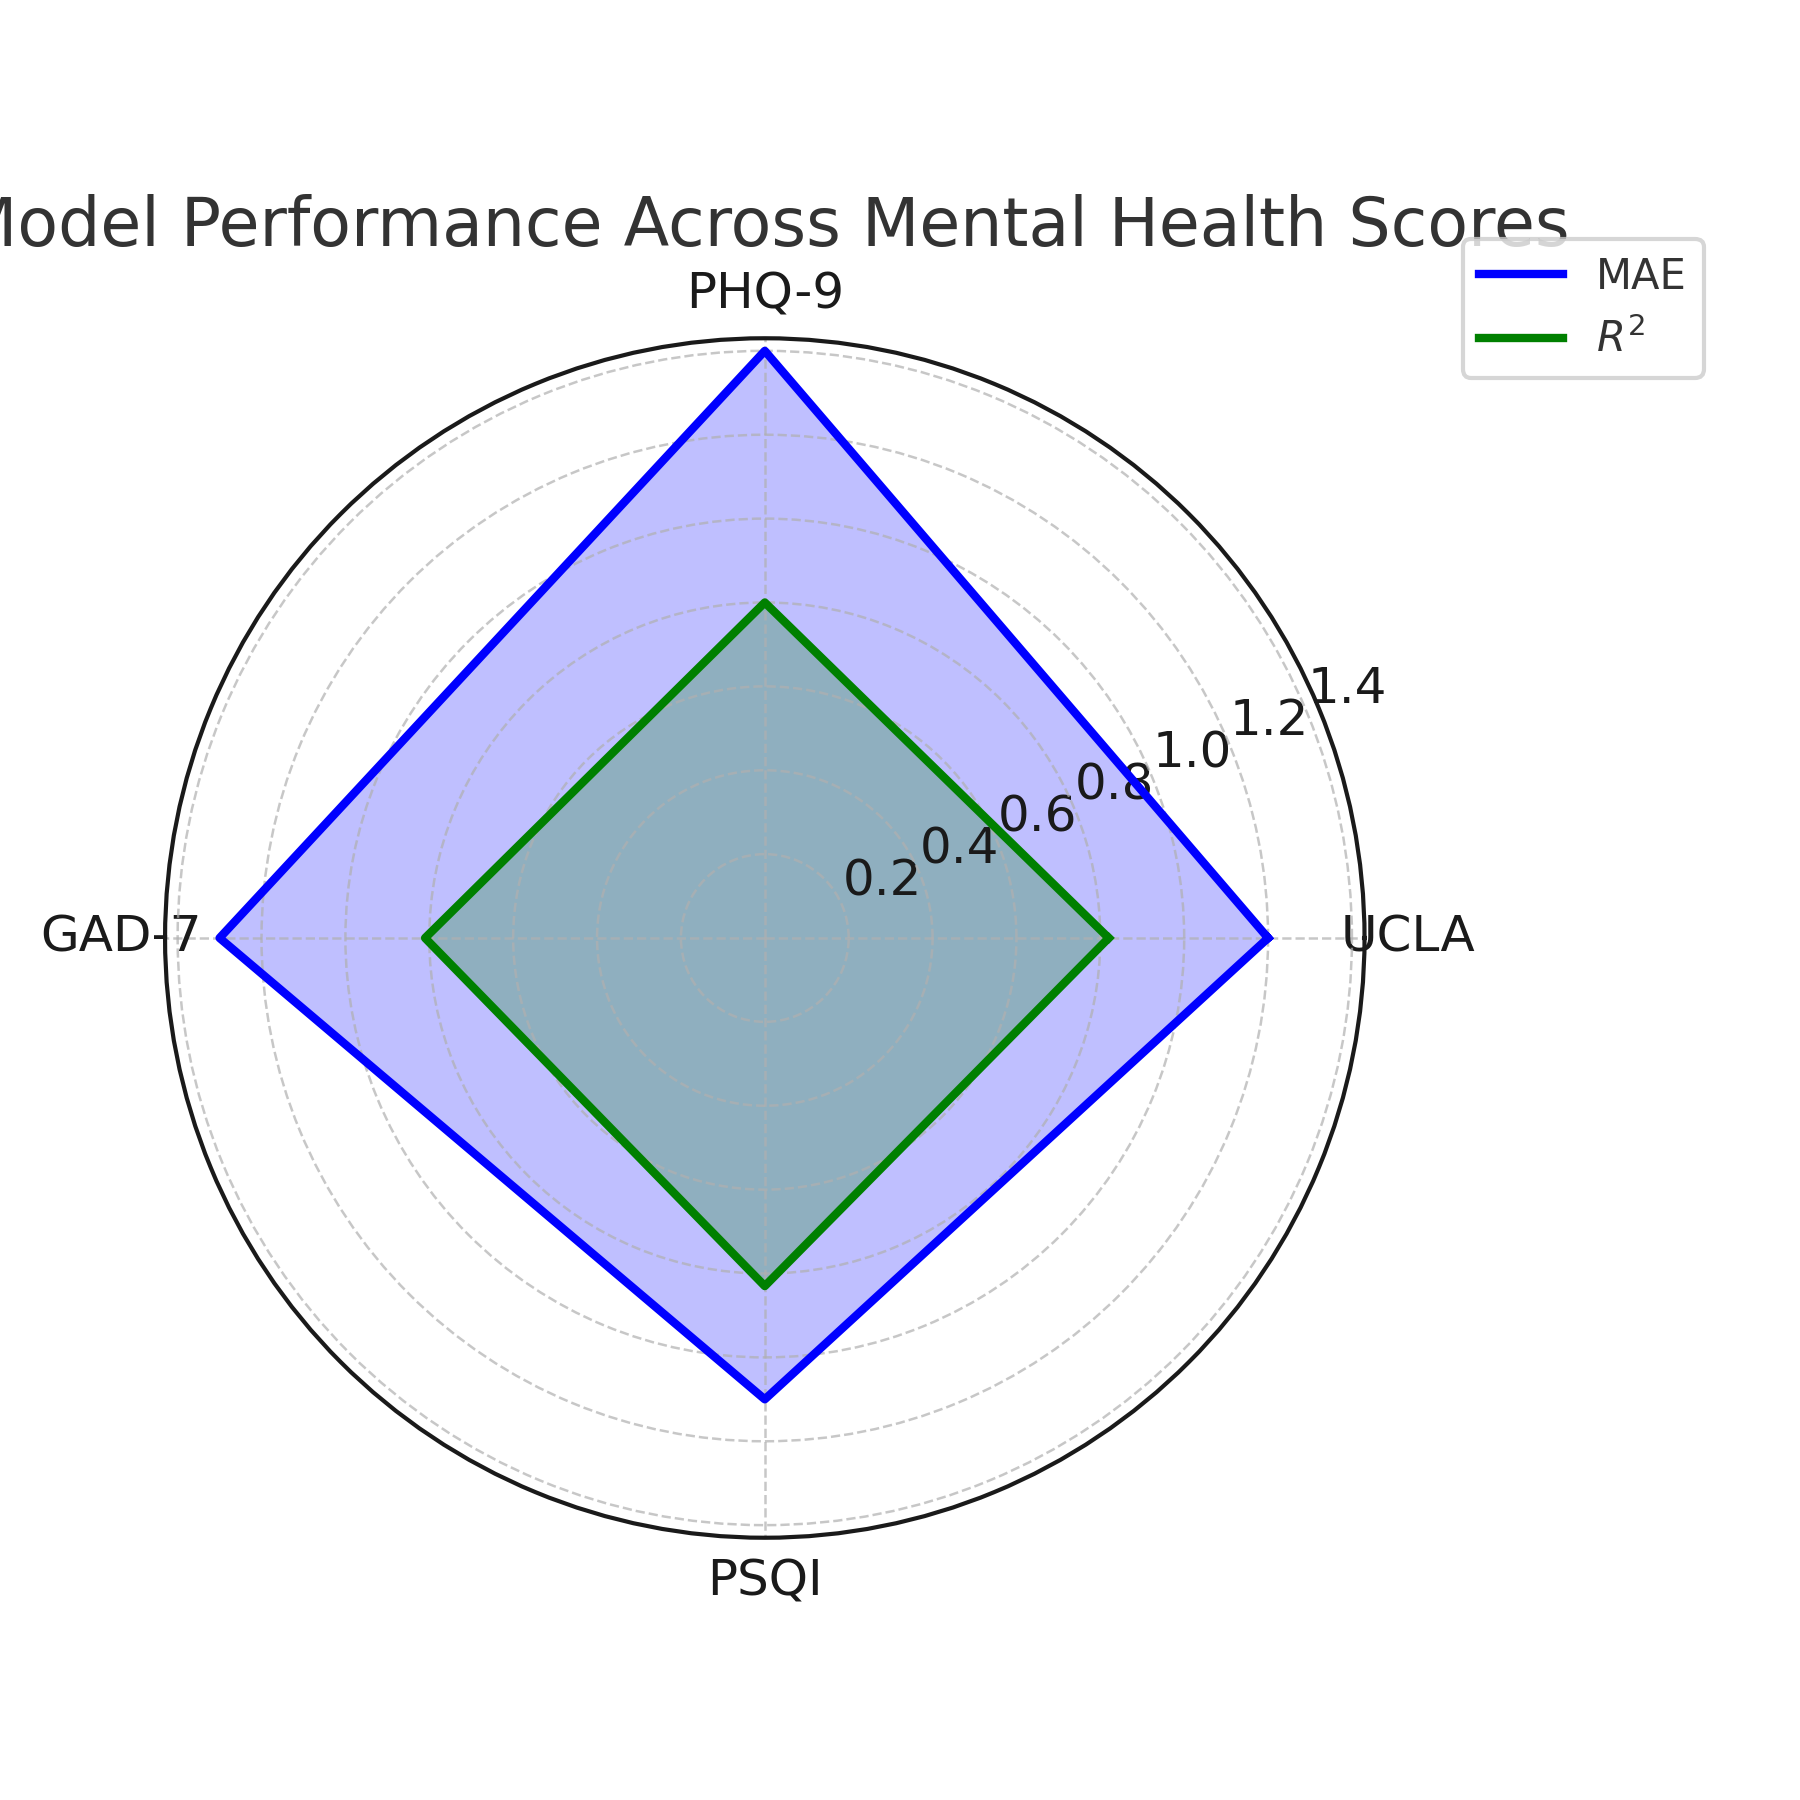
\includegraphics[width=0.45\textwidth]{model_performance_radar.png}
    \caption{Radar chart comparing machine learning model performance (MAE and $R^2$) across UCLA, PHQ-9, GAD-7, and PSQI scores.}
\end{figure}

\textbf{Interpretation:} The radar chart visualizes the performance of machine learning models across the four mental health outcomes (UCLA, PHQ-9, GAD-7, PSQI), comparing two key metrics: mean absolute error (MAE) and explained variance ($R^2$).

All models demonstrate low MAE values (ranging from 1.1 to 1.4), indicating that on average, predicted scores differ from actual scores by about one point. This reflects precise estimation capabilities. Additionally, the $R^2$ values are consistently high (0.80–0.83), meaning that the models explain 80--83\% of the variance in mental health scores.

The nearly symmetric and balanced shape of the radar chart shows that model performance is consistent across all four outcomes, without one scale outperforming or underperforming the others. This suggests that social media behavioral data are broadly predictive, offering robust signals across different psychological dimensions, including loneliness, depression, anxiety, and sleep quality.

Overall, these findings support the conclusion that machine learning models can effectively leverage social media behavior as a non-invasive tool for predicting individual mental health outcomes, opening the door for early screening applications.
\section{Conclusion}
This study demonstrates that social media behavioral data can be leveraged to predict key mental health outcomes, including loneliness (UCLA), depression (PHQ-9), anxiety (GAD-7), and sleep quality (PSQI). Using a combination of correlation analyses, statistical testing, and machine learning models, we showed significant relationships between social media behaviors and psychological scores. Importantly, the machine learning models achieved high predictive accuracy, highlighting the potential of non-invasive digital data streams as mental health screening tools.

\section{Future Work}
While the current study provides promising results, several future directions can enhance its impact:
\begin{itemize}
    \item Incorporating larger and more diverse datasets to improve generalizability across populations.
    \item Exploring additional behavioral and contextual features, such as sentiment analysis of posts or time-of-day activity patterns.
    \item Testing other machine learning architectures, including deep learning models, to improve predictive performance.
    \item Integrating longitudinal data to explore causal relationships and detect early warning signs.
    \item Addressing ethical and privacy concerns when applying predictive models in real-world mental health applications.
\end{itemize}
These future steps will help refine the predictive models and advance the use of social media data in mental health research and clinical interventions.

\bibliographystyle{plain}
\bibliography{references}

\end{document}
